\documentclass[10pt]{beamer}

\usetheme[progressbar=frametitle]{metropolis}
\usepackage{appendixnumberbeamer}

\usepackage{booktabs}

\usepackage{caption}

\usepackage{blindtext}
\usepackage{enumerate}
\usepackage{geometry}

\usepackage{mathtools}
\usepackage{tkz-euclide}
\usepackage{tikz}
\usepackage{xspace}


\title{Theory of Computation}
\subtitle{Tutorial - Pushdown Automata}
\author{Cesare Spinoso-Di Piano}
\date{}

\begin{document}

\maketitle

\begin{frame}{Plan for today}
    \setbeamertemplate{section in toc}[sections numbered]
    \tableofcontents[hideallsubsections]
\end{frame}

\section{What is a Pushdown Automata?}

\begin{frame}{Intuition}

\end{frame}

\section{Formalization}

\begin{frame}{Definition}
    \textbf{Definition.}\footnote{There are many slightly different definitions for PDAs. They are all equivalent in that they all accept exactly the same family of languages.} A nondeterministic pushdown automata (npda) is defined by the seven-tuple $M = (Q, \Sigma, \Gamma, \delta, q_0, z, F)$, where
    \begin{itemize}
        \item $Q$ is a finite set of states
        \item $\Sigma$ is the input alphabet; $\Sigma_\lambda = \Sigma \cup \{\lambda\}$
        \item $\Gamma$ is the stack alphabet; $\Gamma_\lambda = \Gamma \cup \{\lambda\}$
        \item $\delta$: $Q \times \Sigma_\lambda \times \Gamma_\lambda \rightarrow \mathcal{P}_{\texttt{fin}}(Q \times \Gamma^*)$ is the transition function where $\mathcal{P}_{\texttt{fin}}$ is the finite powerset.\footnote{This wasn't necessary for NFAs because the powerset $\mathcal{P}(Q)$ was always finite.}
        \item $q_0\in\Sigma$ is the start state
        \item $z\in\Gamma$ is the stack start symbol
        \item $F \subseteq Q$ is the set of final states
    \end{itemize}
\end{frame}


\begin{frame}{Transition function}
    \textbf{Transition rule.}
    The transition

    $$\delta(q, a, b) = \{(p, c)\}$$

    means while reading an $a \in \Sigma_\lambda$ on your input tape and a $b \in \Gamma_\lambda$ at the top of your stack in the state $q \in Q$ you will transition to state $p \in Q$ and will \textit{replace} $b$ at the top of the stack with $c \in \Gamma_\lambda^*$.

    This is represented graphically as
    \begin{center}
        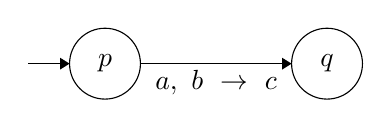
\begin{tikzpicture}[scale=0.15]
            \tikzstyle{every node}+=[inner sep=0pt]
            \draw [black] (25.1,-28.4) circle (3);
            \draw (25.1,-28.4) node {$p$};
            \draw [black] (43.9,-28.4) circle (3);
            \draw (43.9,-28.4) node {$q$};
            \draw [black] (18.6,-28.4) -- (22.1,-28.4);
            \fill [black] (22.1,-28.4) -- (21.3,-27.9) -- (21.3,-28.9);
            \draw [black] (28.1,-28.4) -- (40.9,-28.4);
            \fill [black] (40.9,-28.4) -- (40.1,-27.9) -- (40.1,-28.9);
            \draw (34.5,-28.9) node [below] {$a,\mbox{ }b\mbox{ }\rightarrow\mbox{ }c$};
        \end{tikzpicture}
    \end{center}
\end{frame}

\begin{frame}{Example}
    \textbf{Example.} If we have the transition rule $\delta (q_1, a, b) =\{(q2, cd),(q3, \lambda)\}$, then this is represented graphically as
    \begin{center}
        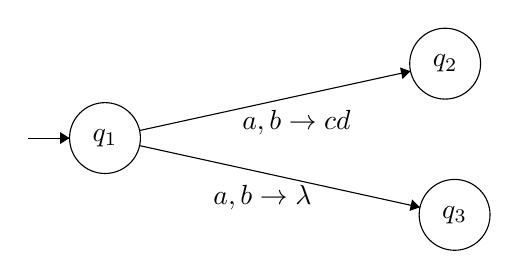
\begin{tikzpicture}[scale=0.15]
            \tikzstyle{every node}+=[inner sep=0pt]
            \draw [black] (19.2,-26.1) circle (3);
            \draw (19.2,-26.1) node {$q_1$};
            \draw [black] (48,-19.8) circle (3);
            \draw (48,-19.8) node {$q_2$};
            \draw [black] (48.8,-32.6) circle (3);
            \draw (48.8,-32.6) node {$q_3$};
            \draw [black] (22.13,-25.46) -- (45.07,-20.44);
            \fill [black] (45.07,-20.44) -- (44.18,-20.12) -- (44.39,-21.1);
            \draw (35.41,-23.69) node [below] {$a,b\rightarrow cd$};
            \draw [black] (12.7,-26.1) -- (16.2,-26.1);
            \fill [black] (16.2,-26.1) -- (15.4,-25.6) -- (15.4,-26.6);
            \draw [black] (22.13,-26.74) -- (45.87,-31.96);
            \fill [black] (45.87,-31.96) -- (45.2,-31.3) -- (44.98,-32.27);
            \draw (32.53,-30.04) node [below] {$a,b\rightarrow\lambda$};
        \end{tikzpicture}
    \end{center}
    \begin{itemize}
        \item From $q_1$ to $q_2$, reading $a$, popping $b$ from the top of the stack and inserting $cd$. \textcolor{red}{The leftmost symbol of $cd$ should be at the top of the stack.}
        \item From $q_1$ to $q_3$, reading $a$ and removing $b$ from the top of the stack
    \end{itemize}
\end{frame}


\begin{frame}{Instantaneous description}
    \textbf{Definition.} The \textbf{instantaneous description} of a PDA $M$ describes the contents of $M$ at a particular instance in its computation. It is a triple $(q, w, u) \in Q \times \Sigma_\lambda^* \times \Gamma_\lambda^*$ where $q$ is the current state, $w$ is the input string left to read and $u$ is the current state of the stack.

    \textbf{Transition rule.} We represent a transition $\delta(q, a, b) = (p, y)$ for the PDA $M$ using instantaneous descriptions as $(q, aw, bx) \succ_M (p, w, yx)$.

    \textbf{Definition.} The language accepted by a PDA $M = (Q, \Sigma, \Gamma, \delta, q_0, z,F)$ is the set
    $$
        L(M) = \{w \in \Sigma^* : (q_0, w, z) \succ_M^* (p, \lambda, u), p \in F, u \in \Gamma^*\}
    $$
\end{frame}

\begin{frame}{Example}
    \textbf{Example.} Consider the following PDA $M$. Suppose $\$$ is the stack start symbol and assume it is already place onto the stack. Let's rune through some computations.

    \begin{center}
        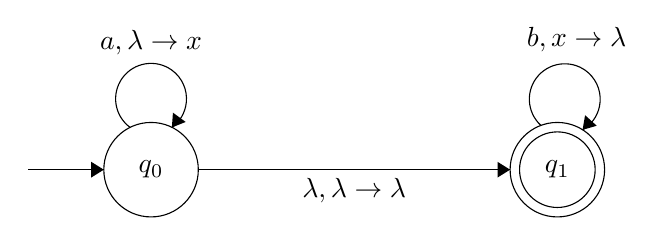
\begin{tikzpicture}[scale=0.2]
            \tikzstyle{every node}+=[inner sep=0pt]
            \draw [black] (21.1,-25.2) circle (3);
            \draw (21.1,-25.2) node {$q_0$};
            \draw [black] (46.9,-25.2) circle (3);
            \draw (46.9,-25.2) node {$q_1$};
            \draw [black] (46.9,-25.2) circle (2.4);
            \draw [black] (45.865,-22.397) arc (227.99099:-60.00901:2.25);
            \draw (48.12,-17.78) node [above] {$b,x\rightarrow\lambda$};
            \fill [black] (48.5,-22.67) -- (49.4,-22.41) -- (48.66,-21.74);
            \draw [black] (24.1,-25.2) -- (43.9,-25.2);
            \fill [black] (43.9,-25.2) -- (43.1,-24.7) -- (43.1,-25.7);
            \draw (34,-25.7) node [below] {$\lambda,\lambda\rightarrow \lambda$};
            \draw [black] (13.3,-25.2) -- (18.1,-25.2);
            \fill [black] (18.1,-25.2) -- (17.3,-24.7) -- (17.3,-25.7);
            \draw [black] (19.777,-22.52) arc (234:-54:2.25);
            \draw (21.1,-17.95) node [above] {$a,\lambda\rightarrow x$};
            \fill [black] (22.42,-22.52) -- (23.3,-22.17) -- (22.49,-21.58);
        \end{tikzpicture}
    \end{center}
\end{frame}

\begin{frame}{Example}
    \textbf{Input String: aabbb}
    \begin{center}
        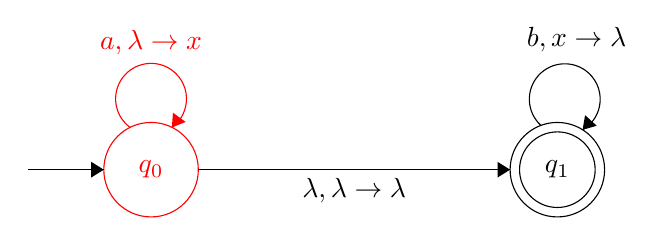
\begin{tikzpicture}[scale=0.2]
            \tikzstyle{every node}+=[inner sep=0pt]
            \draw [red] (21.1,-25.2) circle (3);
            \draw (21.1,-25.2) node {\textcolor{red}{$q_0$}};
            \draw [black] (46.9,-25.2) circle (3);
            \draw (46.9,-25.2) node {$q_1$};
            \draw [black] (46.9,-25.2) circle (2.4);
            \draw [black] (45.865,-22.397) arc (227.99099:-60.00901:2.25);
            \draw (48.12,-17.78) node [above] {$b,x\rightarrow\lambda$};
            \fill [black] (48.5,-22.67) -- (49.4,-22.41) -- (48.66,-21.74);
            \draw [black] (24.1,-25.2) -- (43.9,-25.2);
            \fill [black] (43.9,-25.2) -- (43.1,-24.7) -- (43.1,-25.7);
            \draw (34,-25.7) node [below] {$\lambda,\lambda\rightarrow \lambda$};
            \draw [black] (13.3,-25.2) -- (18.1,-25.2);
            \fill [black] (18.1,-25.2) -- (17.3,-24.7) -- (17.3,-25.7);
            \draw [red] (19.777,-22.52) arc (234:-54:2.25);
            \draw (21.1,-17.95) node [above] {\textcolor{red}{$a,\lambda\rightarrow x$}};
            \fill [red] (22.42,-22.52) -- (23.3,-22.17) -- (22.49,-21.58);
        \end{tikzpicture}
    \end{center}
    \begin{itemize}
        \item Input: \textcolor{red}{a}abbb
        \item Stack: $|\$$
        \item State: $q_0$
    \end{itemize}
\end{frame}

\begin{frame}{Example}
    \textbf{Input String: aabbb}
    \begin{center}
        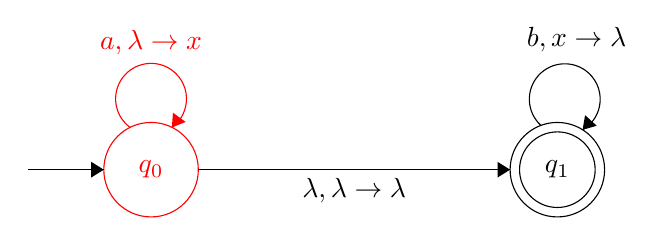
\begin{tikzpicture}[scale=0.2]
            \tikzstyle{every node}+=[inner sep=0pt]
            \draw [red] (21.1,-25.2) circle (3);
            \draw (21.1,-25.2) node {\textcolor{red}{$q_0$}};
            \draw [black] (46.9,-25.2) circle (3);
            \draw (46.9,-25.2) node {$q_1$};
            \draw [black] (46.9,-25.2) circle (2.4);
            \draw [black] (45.865,-22.397) arc (227.99099:-60.00901:2.25);
            \draw (48.12,-17.78) node [above] {$b,x\rightarrow\lambda$};
            \fill [black] (48.5,-22.67) -- (49.4,-22.41) -- (48.66,-21.74);
            \draw [black] (24.1,-25.2) -- (43.9,-25.2);
            \fill [black] (43.9,-25.2) -- (43.1,-24.7) -- (43.1,-25.7);
            \draw (34,-25.7) node [below] {$\lambda,\lambda\rightarrow \lambda$};
            \draw [black] (13.3,-25.2) -- (18.1,-25.2);
            \fill [black] (18.1,-25.2) -- (17.3,-24.7) -- (17.3,-25.7);
            \draw [red] (19.777,-22.52) arc (234:-54:2.25);
            \draw (21.1,-17.95) node [above] {\textcolor{red}{$a,\lambda\rightarrow x$}};
            \fill [red] (22.42,-22.52) -- (23.3,-22.17) -- (22.49,-21.58);
        \end{tikzpicture}
    \end{center}
    \begin{itemize}
        \item Input: a\textcolor{red}{a}bbb
        \item Stack: $x|\$$
        \item State: $q_0$
    \end{itemize}
\end{frame}

\begin{frame}{Example}
    \textbf{Input String: aabbb}
    \begin{center}
        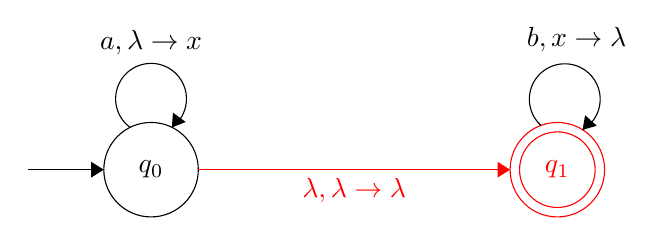
\begin{tikzpicture}[scale=0.2]
            \tikzstyle{every node}+=[inner sep=0pt]
            \draw [black] (21.1,-25.2) circle (3);
            \draw (21.1,-25.2) node {$q_0$};
            \draw [red] (46.9,-25.2) circle (3);
            \draw (46.9,-25.2) node {\textcolor{red}{$q_1$}};
            \draw [red] (46.9,-25.2) circle (2.4);
            \draw [black] (45.865,-22.397) arc (227.99099:-60.00901:2.25);
            \draw (48.12,-17.78) node [above] {$b,x\rightarrow\lambda$};
            \fill [black] (48.5,-22.67) -- (49.4,-22.41) -- (48.66,-21.74);
            \draw [red] (24.1,-25.2) -- (43.9,-25.2);
            \fill [red] (43.9,-25.2) -- (43.1,-24.7) -- (43.1,-25.7);
            \draw (34,-25.7) node [below] {\textcolor{red}{$\lambda,\lambda\rightarrow \lambda$}};
            \draw [black] (13.3,-25.2) -- (18.1,-25.2);
            \fill [black] (18.1,-25.2) -- (17.3,-24.7) -- (17.3,-25.7);
            \draw [black] (19.777,-22.52) arc (234:-54:2.25);
            \draw (21.1,-17.95) node [above] {$a,\lambda\rightarrow x$};
            \fill [black] (22.42,-22.52) -- (23.3,-22.17) -- (22.49,-21.58);
        \end{tikzpicture}
    \end{center}
    \begin{itemize}
        \item Input: aa\textcolor{red}{b}bb
        \item Stack: $xx|\$$
        \item State: $q_0$
    \end{itemize}
\end{frame}

\begin{frame}{Example}
    \textbf{Input String: aabbb}
    \begin{center}
        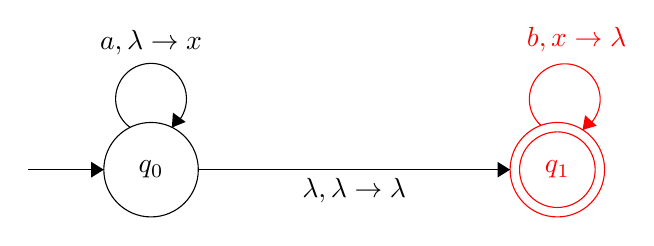
\begin{tikzpicture}[scale=0.2]
            \tikzstyle{every node}+=[inner sep=0pt]
            \draw [black] (21.1,-25.2) circle (3);
            \draw (21.1,-25.2) node {$q_0$};
            \draw [red] (46.9,-25.2) circle (3);
            \draw (46.9,-25.2) node {\textcolor{red}{$q_1$}};
            \draw [red] (46.9,-25.2) circle (2.4);
            \draw [red] (45.865,-22.397) arc (227.99099:-60.00901:2.25);
            \draw (48.12,-17.78) node [above] {\textcolor{red}{$b,x\rightarrow\lambda$}};
            \fill [red] (48.5,-22.67) -- (49.4,-22.41) -- (48.66,-21.74);
            \draw [black] (24.1,-25.2) -- (43.9,-25.2);
            \fill [black] (43.9,-25.2) -- (43.1,-24.7) -- (43.1,-25.7);
            \draw (34,-25.7) node [below] {$\lambda,\lambda\rightarrow \lambda$};
            \draw [black] (13.3,-25.2) -- (18.1,-25.2);
            \fill [black] (18.1,-25.2) -- (17.3,-24.7) -- (17.3,-25.7);
            \draw [black] (19.777,-22.52) arc (234:-54:2.25);
            \draw (21.1,-17.95) node [above] {$a,\lambda\rightarrow x$};
            \fill [black] (22.42,-22.52) -- (23.3,-22.17) -- (22.49,-21.58);
        \end{tikzpicture}
    \end{center}
    \begin{itemize}
        \item Input: aa\textcolor{red}{b}bb
        \item Stack: $xx|\$$
        \item State: $q_1$
    \end{itemize}
\end{frame}

\begin{frame}{Example}
    \textbf{Input String: aabbb}
    \begin{center}
        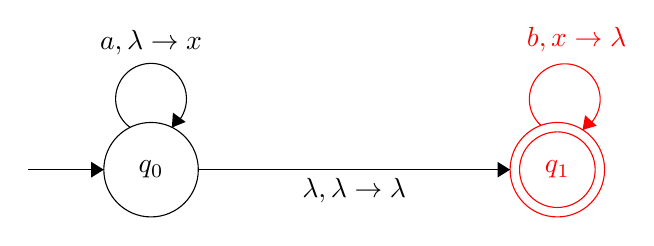
\begin{tikzpicture}[scale=0.2]
            \tikzstyle{every node}+=[inner sep=0pt]
            \draw [black] (21.1,-25.2) circle (3);
            \draw (21.1,-25.2) node {$q_0$};
            \draw [red] (46.9,-25.2) circle (3);
            \draw (46.9,-25.2) node {\textcolor{red}{$q_1$}};
            \draw [red] (46.9,-25.2) circle (2.4);
            \draw [red] (45.865,-22.397) arc (227.99099:-60.00901:2.25);
            \draw (48.12,-17.78) node [above] {\textcolor{red}{$b,x\rightarrow\lambda$}};
            \fill [red] (48.5,-22.67) -- (49.4,-22.41) -- (48.66,-21.74);
            \draw [black] (24.1,-25.2) -- (43.9,-25.2);
            \fill [black] (43.9,-25.2) -- (43.1,-24.7) -- (43.1,-25.7);
            \draw (34,-25.7) node [below] {$\lambda,\lambda\rightarrow \lambda$};
            \draw [black] (13.3,-25.2) -- (18.1,-25.2);
            \fill [black] (18.1,-25.2) -- (17.3,-24.7) -- (17.3,-25.7);
            \draw [black] (19.777,-22.52) arc (234:-54:2.25);
            \draw (21.1,-17.95) node [above] {$a,\lambda\rightarrow x$};
            \fill [black] (22.42,-22.52) -- (23.3,-22.17) -- (22.49,-21.58);
        \end{tikzpicture}
    \end{center}
    \begin{itemize}
        \item Input: aab\textcolor{red}{b}b
        \item Stack: $x|\$$
        \item State: $q_1$
    \end{itemize}
\end{frame}

\begin{frame}{Example}
    \textbf{Input String: aabbb}
    \begin{center}
        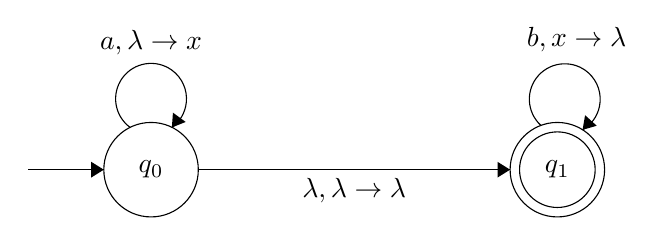
\begin{tikzpicture}[scale=0.2]
            \tikzstyle{every node}+=[inner sep=0pt]
            \draw [black] (21.1,-25.2) circle (3);
            \draw (21.1,-25.2) node {$q_0$};
            \draw [black] (46.9,-25.2) circle (3);
            \draw (46.9,-25.2) node {$q_1$};
            \draw [black] (46.9,-25.2) circle (2.4);
            \draw [black] (45.865,-22.397) arc (227.99099:-60.00901:2.25);
            \draw (48.12,-17.78) node [above] {$b,x\rightarrow\lambda$};
            \fill [black] (48.5,-22.67) -- (49.4,-22.41) -- (48.66,-21.74);
            \draw [black] (24.1,-25.2) -- (43.9,-25.2);
            \fill [black] (43.9,-25.2) -- (43.1,-24.7) -- (43.1,-25.7);
            \draw (34,-25.7) node [below] {$\lambda,\lambda\rightarrow \lambda$};
            \draw [black] (13.3,-25.2) -- (18.1,-25.2);
            \fill [black] (18.1,-25.2) -- (17.3,-24.7) -- (17.3,-25.7);
            \draw [black] (19.777,-22.52) arc (234:-54:2.25);
            \draw (21.1,-17.95) node [above] {$a,\lambda\rightarrow x$};
            \fill [black] (22.42,-22.52) -- (23.3,-22.17) -- (22.49,-21.58);
        \end{tikzpicture}
    \end{center}
    \begin{itemize}
        \item Input: aabb\textcolor{red}{b}
        \item Stack:    \textcolor{red}{$|\$$}
        \item State: $q_1$
    \end{itemize}
    \textcolor{red}{STUCK! Rejected.}
\end{frame}

\begin{frame}{Example}
    What is the language accepted by this PDA?
    \begin{center}
        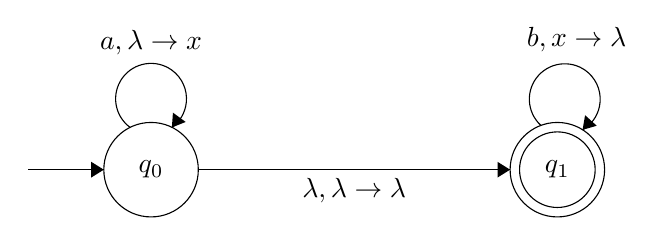
\begin{tikzpicture}[scale=0.2]
            \tikzstyle{every node}+=[inner sep=0pt]
            \draw [black] (21.1,-25.2) circle (3);
            \draw (21.1,-25.2) node {$q_0$};
            \draw [black] (46.9,-25.2) circle (3);
            \draw (46.9,-25.2) node {$q_1$};
            \draw [black] (46.9,-25.2) circle (2.4);
            \draw [black] (45.865,-22.397) arc (227.99099:-60.00901:2.25);
            \draw (48.12,-17.78) node [above] {$b,x\rightarrow\lambda$};
            \fill [black] (48.5,-22.67) -- (49.4,-22.41) -- (48.66,-21.74);
            \draw [black] (24.1,-25.2) -- (43.9,-25.2);
            \fill [black] (43.9,-25.2) -- (43.1,-24.7) -- (43.1,-25.7);
            \draw (34,-25.7) node [below] {$\lambda,\lambda\rightarrow \lambda$};
            \draw [black] (13.3,-25.2) -- (18.1,-25.2);
            \fill [black] (18.1,-25.2) -- (17.3,-24.7) -- (17.3,-25.7);
            \draw [black] (19.777,-22.52) arc (234:-54:2.25);
            \draw (21.1,-17.95) node [above] {$a,\lambda\rightarrow x$};
            \fill [black] (22.42,-22.52) -- (23.3,-22.17) -- (22.49,-21.58);
        \end{tikzpicture}
    \end{center}
\end{frame}

\begin{frame}{Exercise}
    \textbf{Exercise.} What symbols should be in the stack after the following transitions?
    \begin{itemize}
        \item $\delta (q_1, a, \lambda) =\{(q_2, cbb)\}$, Stack: $b|\$$.
        \item $\delta (q_1, a, c) =\{(q_2, \lambda)\}$, Stack: $cb|\$$.
        \item $\delta (q_1, a, \lambda) =\{(q_2, \lambda)\}$, Stack: $cb|\$$.
        \item $\delta (q_1, a, \$) =\{(q_2, \lambda)\}$, Stack: $|\$$.
    \end{itemize}
\end{frame}

\section{Designing PDAs}

\begin{frame}{Tips}
    \begin{itemize}
        \item Use the same pattern matching abilities as DFAs/NFAs,
        \item But now augment this with a stack which can count the occurences of these patterns.
        \item Caveat: You can only use 1 stack and once you read/pop, you can't `go back'.\footnote{This intuitive limitation will be discussed later when we show examples of languages that can't be accepted by PDAs.}
    \end{itemize}
\end{frame}

\begin{frame}[t]{Exercise}
    \textbf{Exercise.} Give a pushdown automata that accepts the language $L=\{a^ib^jc^k|i,j,k\geq 0$ and $i+j=k\}$
\end{frame}

\begin{frame}[t]{Exercise}
    \textbf{Exercise.} Give a pushdown automata that accepts the language $L=\{a^{2n}b^{3n} : n \geq 0 \}$
\end{frame}

\begin{frame}[t]{Exercise}
    \textbf{Exercise.} Give a pushdown automata that accepts the language $\{w \in \{a,b,c\}^* : n_a(w) + n_b(w) \neq n_c(w)\}$
\end{frame}
\end{document}